%SOP Template 
% Version 02 Added revision date
% Version 03 Added TOC and acknowledgements
%           New SOP3_alpha.cls


\documentclass[12pt]{../SOP3}\usepackage[]{graphicx}\usepackage[]{color}
%% maxwidth is the original width if it is less than linewidth
%% otherwise use linewidth (to make sure the graphics do not exceed the margin)
\makeatletter
\def\maxwidth{ %
  \ifdim\Gin@nat@width>\linewidth
    \linewidth
  \else
    \Gin@nat@width
  \fi
}
\makeatother

\definecolor{fgcolor}{rgb}{0.345, 0.345, 0.345}
\newcommand{\hlnum}[1]{\textcolor[rgb]{0.686,0.059,0.569}{#1}}%
\newcommand{\hlstr}[1]{\textcolor[rgb]{0.192,0.494,0.8}{#1}}%
\newcommand{\hlcom}[1]{\textcolor[rgb]{0.678,0.584,0.686}{\textit{#1}}}%
\newcommand{\hlopt}[1]{\textcolor[rgb]{0,0,0}{#1}}%
\newcommand{\hlstd}[1]{\textcolor[rgb]{0.345,0.345,0.345}{#1}}%
\newcommand{\hlkwa}[1]{\textcolor[rgb]{0.161,0.373,0.58}{\textbf{#1}}}%
\newcommand{\hlkwb}[1]{\textcolor[rgb]{0.69,0.353,0.396}{#1}}%
\newcommand{\hlkwc}[1]{\textcolor[rgb]{0.333,0.667,0.333}{#1}}%
\newcommand{\hlkwd}[1]{\textcolor[rgb]{0.737,0.353,0.396}{\textbf{#1}}}%
\let\hlipl\hlkwb

\usepackage{framed}
\makeatletter
\newenvironment{kframe}{%
 \def\at@end@of@kframe{}%
 \ifinner\ifhmode%
  \def\at@end@of@kframe{\end{minipage}}%
  \begin{minipage}{\columnwidth}%
 \fi\fi%
 \def\FrameCommand##1{\hskip\@totalleftmargin \hskip-\fboxsep
 \colorbox{shadecolor}{##1}\hskip-\fboxsep
     % There is no \\@totalrightmargin, so:
     \hskip-\linewidth \hskip-\@totalleftmargin \hskip\columnwidth}%
 \MakeFramed {\advance\hsize-\width
   \@totalleftmargin\z@ \linewidth\hsize
   \@setminipage}}%
 {\par\unskip\endMakeFramed%
 \at@end@of@kframe}
\makeatother

\definecolor{shadecolor}{rgb}{.97, .97, .97}
\definecolor{messagecolor}{rgb}{0, 0, 0}
\definecolor{warningcolor}{rgb}{1, 0, 1}
\definecolor{errorcolor}{rgb}{1, 0, 0}
\newenvironment{knitrout}{}{} % an empty environment to be redefined in TeX

\usepackage{alltt}
%\usepackage[english]{babel}
%\usepackage{blindtext}
%\usepackage{lipsum}

\title{Accumet XL600 Meter}
\date{01/16/2018}
\author{Kate McWilliams}
\approved{Marc Los Huertos}
\ReviseDate{\today}
\SOPno{v.03}
\IfFileExists{upquote.sty}{\usepackage{upquote}}{}
\begin{document}


\maketitle

\section{Scope and Application}

\NP This SOP describes how to use the Accumet meter system to measure and monitor a variety of water-based electrochemical parameters including pH, conductivity, temperature, salinity, dissolved oxygen, and ion-selective mV.

\section{Summary of Method}

\NP Single channel measurements can be made using the Accumet meter. Standardize the pH electrode with buffers that bracket the intended measuring range. Test the pH of a substance using the pH electrode.

\NP Conductivity instructions to be added...
\NP Biological Oxygen Demand instructions to be added...

\tableofcontents

\newpage

\section{Definitions}

\NP Term 1: Electrode- The glass electrodes are ion-selective meaning the glass membrane is sensitive to a specific ion. For example, the pH electrode is sensitive to hydrogen ions. 

\NP Term 2: Buffer- A buffer solution is one which resists changes in pH when small quantities of an acid or an alkali are added to it. Buffer solutions are used as a means of keeping pH at a nearly constant value in a wide variety of chemical applications. 

\section{Biases and Interferences}

\NP Biases and interferences can come from \dots

\section{Health and Safety}

\NP Describe the risk \dots


\subsection{Safety and Personnnel Protective Equipment}


\section{Personnel \& Training Responsibilities}

\NP Researchers training is required before this the procedures in this method can be used\dots 

\NP Researchers using this SOP should be trained for the following SOPs

\begin{itemize}
  \item SOP01 Laboratory Safety
  \item SOP02 Field Safety
\end{itemize}

\section{Required Materials and Apparati}

\NP{Accumet XL600 Benchtop Meter (XL94105590)}
\NP{BOD Probe (2446146 445)} 
\NP{Automatic Temperature Compensation (ATC) Probe (93X306506 505)}
\NP{pH Electrode (13 620 183A)}
\NP{Conductivity Electrode (13 620 100)}
\NP{Standards for calibration (pH 4.00, 7.00, 10.00, conductivity, and a small bottle that can be used to make the DO standard)}

\section{Reagents and Standards}

\NP Buffer Solution pH 4, 7, 10. 
\NP Conductivity Standard 1000$\mu$mho/cm at 25 degrees celsius 

\section{Estimated Time}

\NP This procedure requires XX minutes \dots

\section{Sample Collection, Preservation, and Storage}

\section{Procedure}

\NP To turn on the Accumet, hold the power button for three seconds.
\NP If \emph{Standardization Due Warning} appears, follow the steps in Section 15 to calibrate standard parameters for each measurement type.

\subsection{pH Measurement}
\NP If the pH electrode has been stored dry, soak in storage solution for 10 minutes before standardization to saturate the pH electrode surface and minimize drift. If storage solution is not available, use a neutral pH buffer. While okay for rinsing, do not store pH electrodes in deionized or distilled water as this will dehydrate the electrode and decrease performance.
\NP In the single channel measurement display of pH, select the Measurement icon on the right-side menu. A graph will appear and begin tracking pH.
\NP Fill the outer cavity with the liquid you wish to measure and stir gently to speed up the response and permit a more representative measurement.
\NP After measurement, remove the electrode from the sample rinse with clean water. Do not wipe the electrode. This may impart a static charge, and result in an unstable reading. A hydrated electrode is important– rinse and shake dry without wiping, and place the electrode into your storage solution.
\NP When you are finished, fill outer cavity with pH Electrode Storage Solution.
\NP See section 15 to learn how to standardize the pH parameters.

\subsection{Temperature Measurement}
\NP The ATC probe eliminates errors calculating pH. This is necessary because accuracy of the pH probe decreases as samples deviate from 25 degrees C and pH 7. If you are not using an ATC probe, the default temperature (25 degrees C) will be used instead. The default temperature range is -10 degrees C to 110 degrees C. 
\NP If  you  are measuring the  pH  of  a  solution  that  is  not  25 degrees C  and  you  are  not  using  an (ATC)  probe, enter  the  temperature  value  of  the  solution  for  best  results.
The manual temperature compensation (MTC) value will be visible on the screen. The default temperature can be set from -5 degrees C to 105 degrees C.
\NP\textbf{Set Default Temperature}. First, select temperature units \textbf{C} Celsius, \textbf{F} Farenheit, or \textbf{K} Kelvin. Then Touch the \textbf{Default Temperature} box and use the numeric keypad to enter the desired default temperature.
Press \textbf{Enter} in the keypad to return to pH (pH FET) Setup screen


\subsection{BOD (Biological Oxygen Demand) Measurement}
\NP To Be Added...

\subsection{Conductivity Measurement}
\NP TBA...


\section{Data Analysis and Calculations}

\subsection{Graphing pH}
\NP The efficiency of the electrode is reported as the slope. Slope can be described as percentage where 100\% is ideal, or as a mV/decade unit. When performing  standardization with 3 or more standards, multiple slopes will be calculated by the  instrument. The slope that appears on the screen during measurement, is the slope which is applicable to the zone in which the measurement is currently being made. For example, if pH 4, 7, and 10 are standardized, and a sample of pH 5 is being measured, the slope displayed would be the slope calculated between 4 and 7. The slopes are independent of each other. 

\NP Real-time data can be viewed on a graph to view changes over brief or  extended  periods. Time  is  plotted  in  seconds. The  graph  refreshes  every  hour  from  the  start of graphing.
\NP Select Show Graph. A graph will be displayed on the lower half of the screen where various measurement details were previously displayed.  
\NP To track live measurement data on the graph, select 
Start Plotting. The measurement data will continue until 
Stop Plotting is selected. When stopped, the graph can be dragged left/right and up/down.
\NP Select the Zoom In or Zoom Out options to examine the data more closely or broadly.
\NP To remove the graph display and revert to display measurement data on the lower half of the screen, select Hide Graph. Note:Measurement  data  will  continue  to  be  tracked  on  the  graph  until  Stop  Plotting is  selected.  

\section{QC/QA Criteria}

\section{Trouble Shooting}

\subsection{No response or all buffers read the same pH}

\NP Verify that the correct meter input and channels are connected. Try removing the electrode storage bottle or rubber bulb guard to ensure contact with sample. If the meter has automatically frozen reading, be sure the meter's hold or auto read feature are off. Lastly, try replacing the electrode.  

\subsection{Slow electrode response with excessive crystallization inside the electrode}

\NP Verify that the fill hole is open durign measurements and closed during storage. Otherwise, the electroclyte flow could be clogged with supersaturated electrolyte. Flush and refill electrode. Remove the filling solution through the fill hole with a syringe or by shakign it upside down. Repeatedly flush and rinse the reference cavity with clean water at a temp of 60-80 degrees celsius to dissolve crystals. Replace the filling solution and apply gentle pressure to filling hole. Hydrate the electrode in storage solution.

\subsection{Slow electrode response due to clogged junction}

\NP For protein deposits, prepare a 1\% pepsinsolution in 0.1M HCI and soak the reference junction for one hour. Rinse the electrode with distilled water. For general cleaning, heat a diluted KCI solution to 60 to 80 degrees celsius and soak the sensing bulb for about 10 minutes. All the electrode to coll in unheated KCI solution.

\subsection{Dried Salt Deposits}

\NP Dissolve the salt deposits in warm tap water and then soak the electrode briefly in pH 4 buffer.

\subsection{Slow electrode response, noisy, unstable or eratic readings}

\NP Clean the electrode with mild detergent and warm water and then hydrate. Allow the electrode to reach sample temp. Take 30 minute readings and soak the electrode in pH buffer for 1 minute between measurements.

\section{Calibration}

\subsection{Temperature Probe}

\NP Connect the ATC probe and place it into a solution with a known accurate temperature such as a constant temperature bath.

\NP When the temperature reading is stable, select Standardize from any measure screen, and then select the Temp Std. icon. The upper display shows the current factory default temperature without standardization (A), while the lower display will be the new standardization temperature(B).

\NP To enter a new Standardization Temperature, select the box and enter value using the keypad that will appear. Select OK to accept the new temperature.

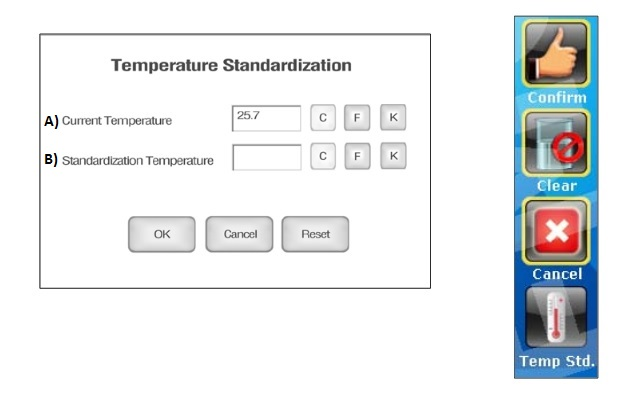
\includegraphics{Tempstandard.jpg}

\subsection{pH Probe}

\NP In PH Setup, select the buffer group custom, as this allows manual buffer recognition. There is an option for autodetection for setting parameters, but in this course we will only use manual.
\NP Back at the pH measurement display, select \textbf(Standardize) at the top right.
\NP If the pH electrode has been stored dry, soak in storage solution for 10 minutes before standardization to saturate the pH electrode surface and minimize drift. If storage solution is not available, use a neutral pH buffer. While OK for rinsing, do not store pH electrodes in deionized or distilled water as this will dehydrate the electrode and decrease performance. 
\NP Fill outer cavity with the first standard, pH 4. The level of electrolyte in the outer cavity should be kept above the level of the solution being measured to prevent reverse electrolyte flow. The electrolyte need only be immersed far enough to cover both the glass pH sensing bulb and reference junction (see diagram below) to obtain accurate readings.
\NP Enter pH value in the keypad on the screen.
\NP When dispay reads \textbf(Stable), select \textbf{Confirm} to accept the value and return to measurement screen. A warning message will appear if the standardization is accepted by the instrument but is not within range. An error message will appear if the standardization is not accepted.
\NP Now dispose of the buffer in the outer cavity and rinse the cavity and electrode. Repeat from step... to input standards pH 7 and pH 10.
\NP When you are finished, fill outer cavity with pH Electrode Storage Solution.

\NP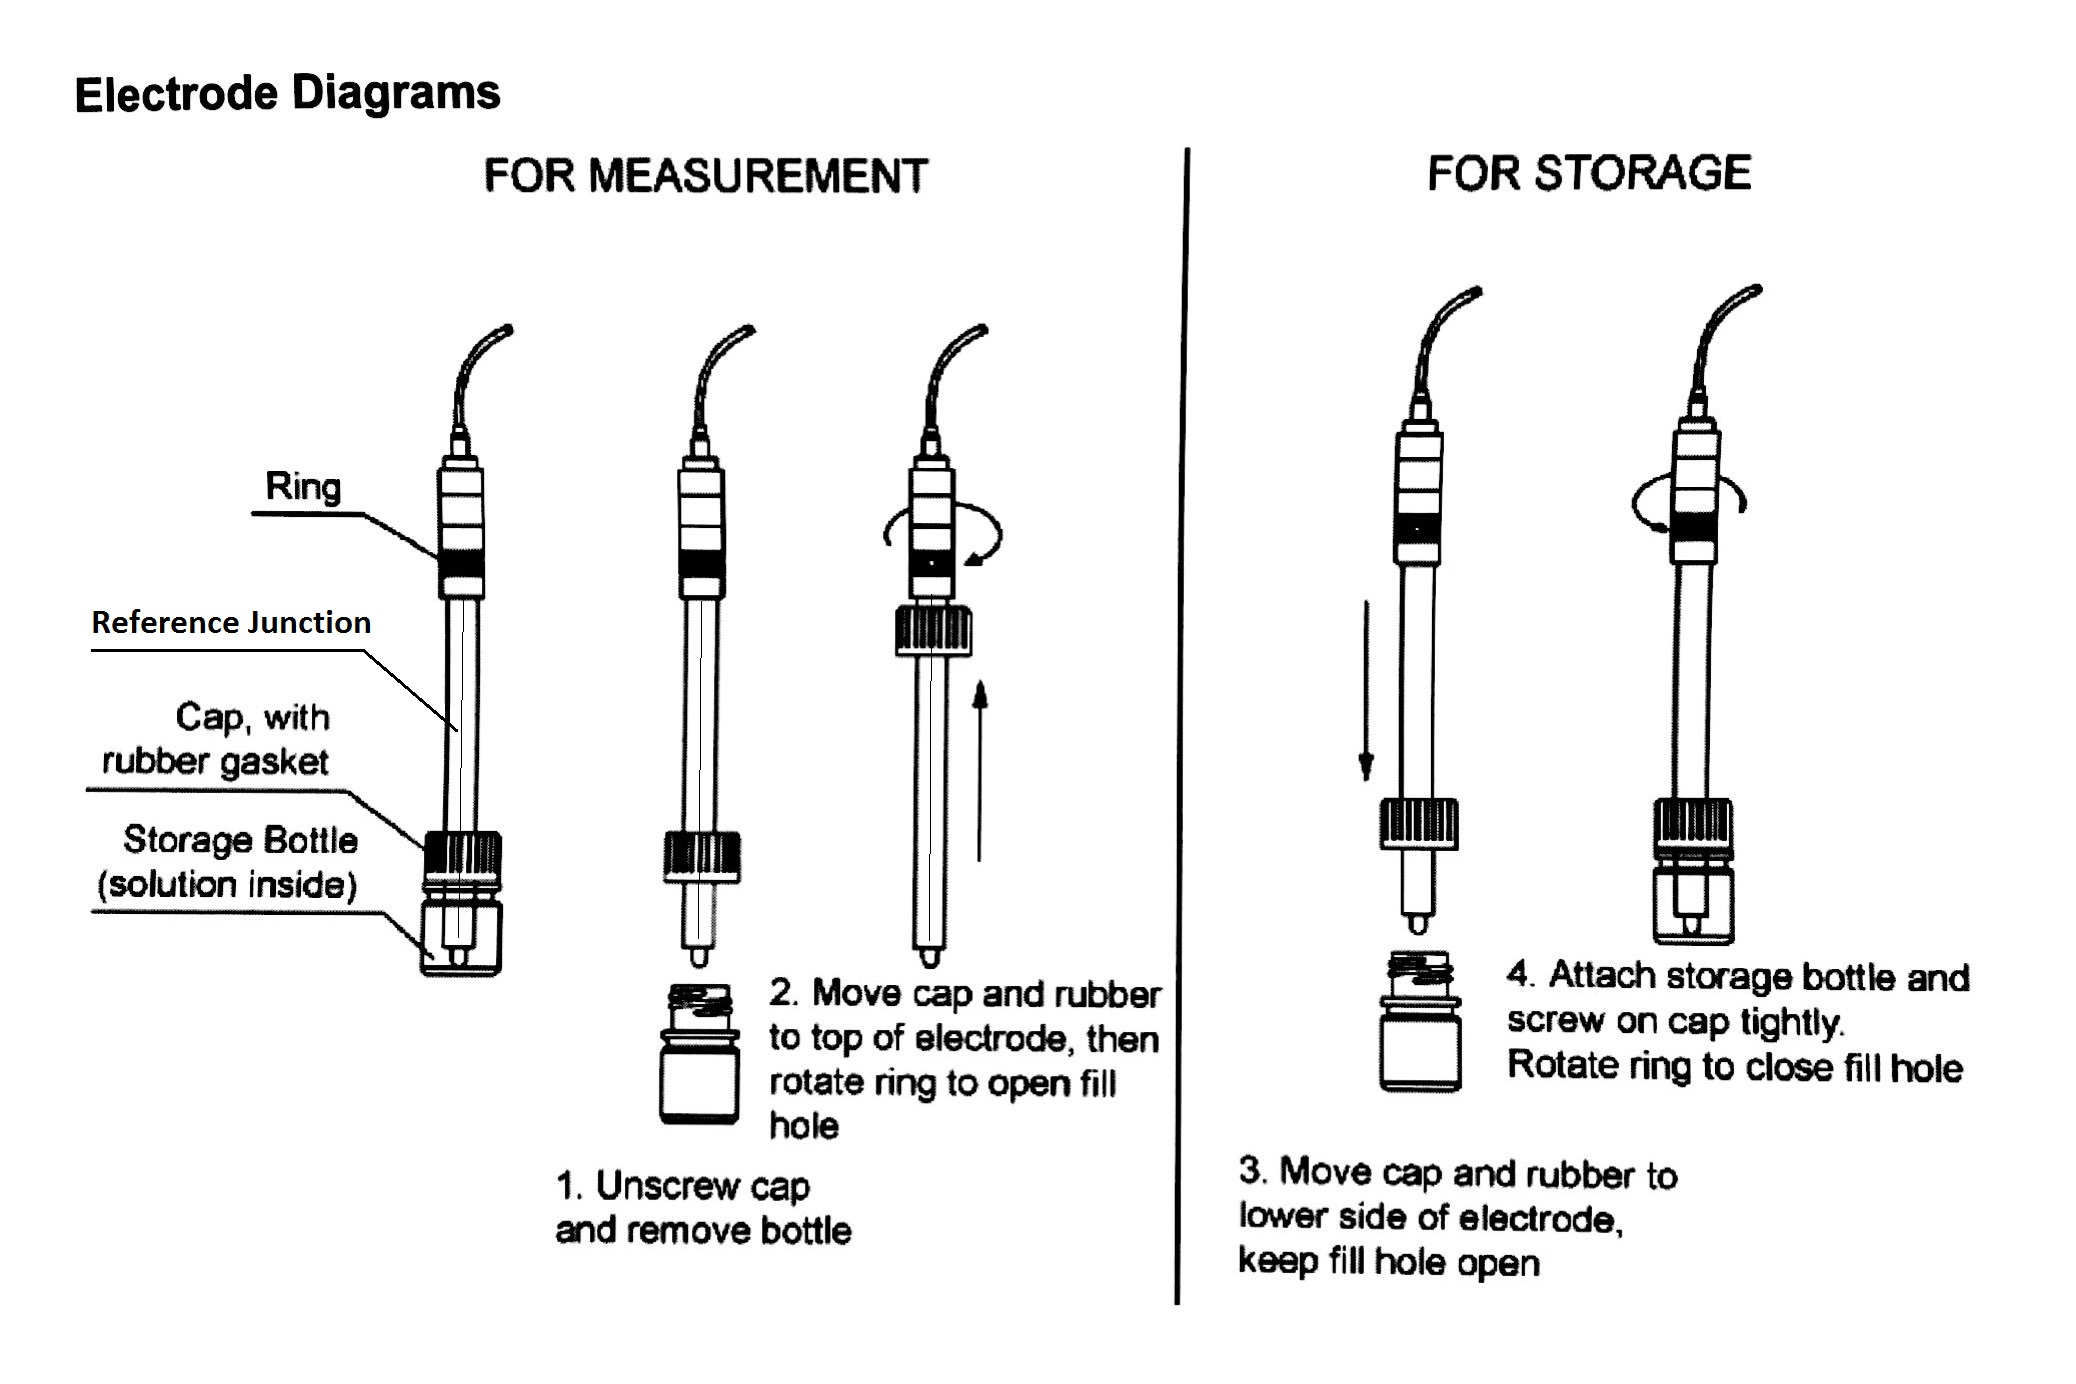
\includegraphics[scale=.25]{Electrode.jpg}

\subsection{Conductivity}

\NP In Conductivity Setup, select MANUAL to enter the conductivity value of your standard. You may set \textbf{Single Point Standardization} in which the single standard applies to all ranges, or \textbf{Multi Point Standardization} in which a single stard is applied to an specific range. When using a Multi Point standardization, perform standardization in each range that you expect to use for best results.
\begin{figure}
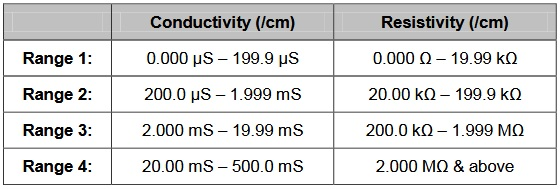
\includegraphics{Conducivityranges.jpg}
\end{figure}
\NP{Cell Constant.} Select the nominal cell constant of the conductivity electrode you are using. There are three cell constants to choose from. Each is used for a different range. The following indicates the optimal conductivity range for the accumet conductivity cells. For resistivity measurements, an electrode having a nominal 0.1 cell constant (13-620-101 or equivalent) is recommended.
\begin{figure}
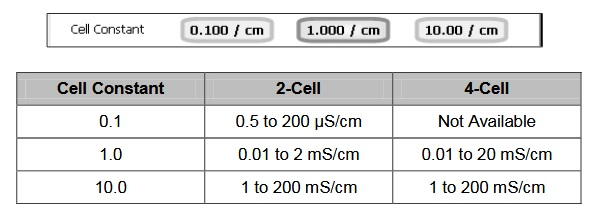
\includegraphics{CellConstant.jpg}
\end{figure}
\section{References}

\NP APHA, AWWA. WEF. (2012) Standard Methods for examination of water and wastewater. 22nd American Public Health Association (Eds.). Washington. 1360 pp. (2014).

\NP Online Instruction Manual can be found here: link

\end{document}
